\documentclass[11pt,a4paper,openright,twoside]{article}
\usepackage[english]{babel}
\usepackage{newlfont}
\usepackage{color}
\textwidth=450pt\oddsidemargin=0pt
\usepackage{graphicx}
\usepackage{float}
\usepackage{textcomp}
\usepackage{caption}
\usepackage{wrapfig}
\usepackage{subfig}
\usepackage{sidecap}
\usepackage[rlft]{floatflt}
\usepackage{amsmath}
\usepackage{amssymb}
\usepackage{bm}
\usepackage{fancyhdr}
\usepackage{multirow}
\usepackage[utf8x]{inputenc}
\usepackage{fullpage}
\usepackage[Lenny]{fncychap}
\usepackage[T1]{fontenc}
\usepackage[normalem]{ulem}
\usepackage{booktabs}
\usepackage{enumerate}
\usepackage{tikz}
\usetikzlibrary{positioning}

\tikzset{c-rectangle2/.style={rectangle, rounded corners, minimum width=2cm, minimum height=1cm, text centered, text width=4cm, draw=black, fill=white},
arrow/.style={thick,->,>=stealth}}

%\usepackage[usenames,dvipsnames]{xcolor}
%\usepackage{listings}
%\usepackage{xcolor}

%\definecolor{light-gray}{gray}{0.95}
%\lstset{language=R,
%    basicstyle=\small\ttfamily,
%    stringstyle=\itshape\color{RedViolet},
%    showstringspaces=false,
%    otherkeywords={0,1,2,3,4,5,6,7,8,9},
%    morekeywords={TRUE,FALSE, ggplot, data.frame, theme, ylab, xlab},
%    deletekeywords={data, frame, beta, c, par, colours, contour, scale,
%                    panel, grid, hat},
%    keywordstyle=\color{RoyalBlue},
%    commentstyle=\itshape\color{PineGreen},
%    backgroundcolor=\color{light-gray}
%}

\title{Permutation Closed Testing with Sum-Based Statistics}
\author{}
\date{}





\begin{document}

\maketitle


\section{Sum-Based Test Statistics}
Given a full model $F=\{1,\ldots, f\}$ of univariate hypotheses, let $S\subseteq F$ be a subset under test by closed testing with level $\alpha$. Hence $S$ is rejected if and only if all its supersets $S\cup V$ ($V\subseteq F\setminus S$) are rejected.

Let
\[g_i^\pi\quad (i=1,\ldots,f,\; \pi=1,\ldots,B)\]
be some test statistics corresponding to the $f$ covariates and $B$ random permutations, where the first permutation is the identity. Assume that the null hypothesis is rejected for high values of $g_i$ (otherwise, it is sufficient to multiply all test statistics by $-1$), and
\[g_V^\pi=\sum_{i\in V}g_i^\pi\quad (V\subseteq F,\;\pi=1,\ldots,B).\]
Moreover, define the centered test statistics
\[d_i^\pi = g_i^\pi - g_i \quad (i=1,\ldots,f,\; \pi=1,\ldots,B),\]
so that the observed values are all $d_i=0$, and the variability due to $g_i$ is excluded.

For $V\subseteq F$, the vector of its statistics is
\[\mathbf{d_V}=(0,d_V^2,\ldots,d_V^B)^\top.\]
Consider the sorted test statistics $d_V^{(1)}\leq d_V^{(2)}\leq\ldots\leq d_V^{(B)}$, and define $k=\lceil (1-\alpha) B\rceil$. The permutation test rejects $V$ if
\[d_V^{(k)}< 0.\]
Such a test can be slightly conservative, but it can be adapted to be exact by randomizing it.







\vspace{10mm}

\section{Shortcut}
Let $s=|S|$ and $m=f-s$, and fix a value $v\in\{0,\ldots,m\}$. We will define a shortcut for the analysis of the supersets $S\cup V$ with $V\in\mathcal{V}_v$ and
\[\mathcal{V}_v=\{V\,:\,V\subseteq F\setminus S,\; |V|=v\},\]
that does not require all the $\binom{m}{v}$ vectors $\mathbf{d}_{V}$. It relies on the construction of a lower and an upper critical values, $L_v$ and $U_v$, such that
\begin{itemize}
\item if $L_v\geq 0$, then at least one superset $S\cup\tilde{V}$ is not rejected, and thus $S$ is not rejected;
\item if $U_v<0$, then all supersets are rejected, and other sizes can be explored.
\end{itemize}
Notice that if $L_v< 0\leq U_v$, then the outcome is indecisive. 


\paragraph{Lower critical value.} In order not to reject $S$, it is sufficient to find a non-rejected superset. We define the lower critical value as $L_v=(d_{S} + l_v)^{(k)}$, where $\mathbf{l}_v=\mathbf{d}_{\tilde{V}}$ and $\tilde{V}\in\mathcal{V}_v$ is such that $S\cup\tilde{V}$ is likely to be non-rejected.

In particular, $\tilde{V}$ is defined by considering the indices of the $v$ smallest observed statistics not in $S$. If $(i_1,\ldots,i_m)$ is a permutation of the indices in $F\setminus S$ such that
\[g_{i_1}\leq g_{i_2}\leq\ldots\leq g_{i_m},\]
then $\tilde{V}=\{i_1,\ldots,i_v\}$ and
\[l_v^\pi = \sum_{h=1}^v d_{i_h}^\pi\quad (\pi=1,\ldots,B).\]



\paragraph{Upper critical value.} The upper critical value is $U_v=(d_{S} + u_v)^{(k)}$, where
\[\mathbf{u}_v=(0,u_v^2,\ldots,u_v^B)^\top\]
is a vector such that
\[u_v^\pi\geq d_V^\pi\quad (V\in\mathcal{V}_v,\;\pi=1,\ldots,B).\]
As a consequence,
\[U_v \geq (d_S + d_V)^{(k)}\quad (V\in\mathcal{V}_v).\]
If $U_v<0$, then all supersets $S\cup V$ with $V\in\mathcal{V}_v$ are rejected.

For each $\pi=1,\ldots,B$, the element $u_v^\pi$ is defined by considering the $v$ highest centered statistics not in $S$. If $(j_1(\pi),\ldots,j_m(\pi))$ is a permutation of the indices in $F\setminus S$ such that
\[d_{j_1(\pi)}^\pi\geq d_{j_2(\pi)}^\pi\geq\ldots d_{j_m(\pi)}^\pi ,\]
then
\[u_v^\pi=\sum_{h=1}^v d_{j_h(\pi)}^\pi.\]




\paragraph{Testing.}
The values $v=0,\ldots, m$ are checked in sequence.
\begin{itemize}
\item As soon as a non-rejection is found (there exists $v^*$ such that $L_{v^*}\geq 0$), the analysis stops and $S$ is not rejected.
\item If all values lead to rejection ($U_v<0$ for all $v$), then $S$ is rejected.
\item If some values $v\in \{1,\ldots,m-1\}$ lead to indecisive outcomes ($L_v < 0\leq U_v$), the Branch and Bound method is applied. Notice that an indecisive outcome cannot occur for $v=0$ or $v=m$, since
\begin{align*}
& L_0=U_0=d_S^{(k)} & L_m=U_m=d_F^{(k)}.
\end{align*}
\end{itemize}



\paragraph{Early stop.} Assume that there exists $w\in\{1,\ldots,m\}$ such that all the elements of $\textbf{u}_w$ are smaller than those of $\textbf{u}_{w-1}$:
\[u_w^\pi =u_{w-1}^\pi +d_{j_w(\pi)}^\pi\leq u_{w-1}^\pi\quad (\pi=1,\ldots,B)\]
or, equivalently,
\[d_{j_w(\pi)}^\pi\leq 0\quad (\pi=1,\ldots,B).\]
Then the upper critical value is non-increasing for $v\geq w$:
\begin{align*}
d_{j_m(\pi)}^\pi\leq \ldots \leq d_{j_w(\pi)}^\pi \leq 0&\quad(\pi=1,\ldots,B)\\
u_m^\pi \leq\ldots\leq u_w^\pi\leq u_{w-1}^\pi&\quad(\pi=1,\ldots,B)\\
U_m \leq\ldots\leq U_w\leq U_{w-1}. &
\end{align*}

In this case, it is sufficient to stop the analysis as soon as we find a value $v^*\geq w-1$ such that $U_{v^*}<0$. All the supersets with $v\geq v^*$ are automatically rejected.





\vspace{10mm}

\section{Branch and Bound}
Assume that some values $v\in\{1,\ldots,m-1\}$ lead to an indecisive outcome. 

For a fixed index $e\in F\setminus S$, the total space $\mathbb{S}=\{V\,:\,V\subseteq F\setminus S\}$ is partitioned into two disjoint subspaces, according to the inclusion of $e$:
\begin{align*}
&\mathbb{S}_{-e}=\{V\,:\,V\subseteq F\setminus(S\cup\{e\})\} & \mathbb{S}_{+e}=\{V\,:\,\{e\}\subseteq V\subseteq F\setminus S\}.
\end{align*}

The shortcut is applied to each subspace, in order to evaluate the indecisive values $v$:
\begin{itemize}
\item if $S$ is not rejected in at least one subspace, it is not rejected in the total space;
\item if $S$ is rejected in both subspaces, it is rejected in the total space;
\item if there is an indecisive outcome in at least one subspace, the procedure is iterated by partitioning the indecisive subspace(s).
\end{itemize}

For any choice of $e$, $U_v$ does not increase in the subspaces (since it is defined by taking the maximum statistics over smaller subsets). However, the choice of $e$ and the order in which the subspaces are explored influence $L_v$, and thus the efficiency of the algorithm. We wish to begin with the subspaces that are more likely to lead to a non-rejection, i.e. where $L_v$ is more likely to be high.

We will evaluate the efficiency in four different scenarios, employing the order of the observed statistics in $F\setminus S$. The scenarios differ by the index $e$ used for branching:
\begin{itemize}
\item highest statistic $e=i_m$ ($L_v$ does not vary in $\mathbb{S}_{-e}$);
\item lowest statistic $e=i_1$ ($L_v$ does not vary in $\mathbb{S}_{+e}$).
\end{itemize}
Moreover, they differ by the branch that is explored first:
\begin{itemize}
\item $\mathbb{S}_{-e}$, removal;
\item $\mathbb{S}_{+e}$, keeping.
\end{itemize}
Preliminary simulations suggest that removing the highest statistic could lead to the smallest number of iterations in most cases.









\newpage

\section{Example}
Considering $f=5$ predictors and $B=10$ permutations, we simulate a $B\times f$ matrix of global test statistics:

\begin{table}[h!]
\centering
\begin{tabular}{ccccc}
\multicolumn{5}{c}{$\mathbf{G}$}\\
$(1)$ & $(2)$ & $(3)$ & $(4)$ & $(5)$\\
\cline{1-5}
28.42 & 16.68 & 9.36 & 6.12 & 9.40\\
0.10 & 0.06 & 1.37 & 0.08 & 0.56\\
0.69 & 3.07 & 4.33 & 0.83 & 0.36\\
1.07 & 30.31 & 1.11 & 8.55 & 0.26\\
0.22 & 7.45 & 2.87 & 0.48 & 1.02\\
1.83 & 0.04 & 2.85 & 0.04 & 0.02\\
17.68 & 1.82 & 6.00 & 1.52 & 1.06\\
1.77 & 26.12 & 0.29 & 0.26 & 4.07\\
2.71 & 0.37 & 8.47 & 5.83 & 4.42\\
1.14 & 0.03 & 24.06 & 8.84 & 2.41\\
\end{tabular}
\end{table}

Assume that we want to test $S=\{5\}$ with significance level $\alpha=0.20$.




\paragraph{Shortcut.}
\begin{table}[h!]
\centering
\resizebox{\textwidth}{!}{
\begin{tabular}{c|ccccccccccc}
v &   &  &  &  &  &  &  &  &  &  &  \\
4 &  &  &  &  &  & $\mathbf{F=\{1,2,3,4,5\}}$ &  &  &  &  &  \\
3 &  &  & $\{1,2,3,5\}$ &  & $\{1,2,4,5\}$ &  & $\{1,3,4,5\}$ &  & $\mathbf{\{2,3,4,5\}}$ &  &  \\
2 & $\{1,2,5\}$  &  & $\{1,3,5\}$ &  & $\{1,4,5\}$ &  & $\{2,3,5\}$ &  & $\{2,4,5\}$ &  & $\mathbf{\{3,4,5\}}$ \\
1 &  &  & $\{1,5\}$ &  & $\{2,5\}$ &  & $\{3,5\}$ &  & $\mathbf{\{4,5\}}$ &  &  \\
0 &  &  &  &  &  & $\mathbf{S=\{5\}}$ &  &  &  &  &  
\end{tabular}
}
\caption{Supersets of $S=\{5\}$by size. The sets in bold are used to define the lower critical value $L_v$.}
\end{table}

We define
\begin{itemize}
\item $\mathbf{D}$, matrix of the centered test statistics in $F\setminus S$, where the indices appear in the order $(4,3,2,1)$ (since $g_4\leq g_3\leq g_2\leq g_1$);
\item $\mathbf{R}$, matrix obtained from $\mathbf{D}$ by sorting the elements within each row in decreasing order;
\item $\mathbf{Dsum}$ and $\mathbf{Rsum}$, matrices of the cumulative sums of $\mathbf{d}_S$ with $\mathbf{D}$ and $\mathbf{R}$, respectively.
\end{itemize}

Let $k=\lceil (1-\alpha) B\rceil =8$. The lower and upper critical values, $L_v$ and $U_v$, are the $k$-th ordered statistics of
\begin{align*}
& \mathbf{d}_S +\mathbf{l}_{v}=\mathbf{Dsum}_{v+1} & \mathbf{d}_S + \mathbf{u}_v=\mathbf{Rsum}_{v+1}.
\end{align*}

The first column of $\mathbf{R}$ having no positive elements has index $w=3$. We start by computing both bounds for $v=0,1,2$. No non-rejection is found, but the values $v=1,2$ lead to an indecisive outcome.

We proceed by examining $v>2$, until we find either a rejection or a negative $U_v$. Since $U_v$ becomes negative for $v=3$, the supersets with $v=3,4$ are automatically rejected.


\newpage

\begin{table}[h!]
\centering
%\resizebox{\textwidth}{!}{
\begin{tabular}{ccccccccccc}
$\mathbf{d}_S$ & & \multicolumn{4}{c}{$\mathbf{D}$} & & \multicolumn{4}{c}{$\mathbf{R}$}\\
$(5)$ &  & $(4)$ & $(3)$ & $(2)$ & $(1)$ &  &  &  &  &  \\
\cline{1-1} \cline{3-6} \cline{8-11}
0.00 &  & 0.00 & 0.00 & 0.00 & 0.00 &  & 0.00 (1)& 0.00 (2)& 0.00 (3)& 0.00 (4)\\
-8.84 &  & -6.03 & -7.99 & -16.62 & -28.32 &  & -6.03 (4)& -7.99 (3)& -16.62 (2)& -28.32 (1)\\
-9.04 &  & -5.29 & -5.02 & -13.61 & -27.72 &  & -5.02 (3)& -5.29 (4)& -13.61 (2)& -27.72 (1)\\
-9.14 &  & 2.43 & -8.25 & 13.63 & -27.34 &  & 13.63 (2)& 2.43 (4)& -8.25 (3)& -27.34 (1)\\
-8.38 &  & -5.63 & -6.49 & -9.23 & -28.19 &  & -5.63 (4)& -6.49 (3)& -9.23 (2)& -28.19 (1)\\
-9.38 &  & -6.08 & -6.51 & -16.64 & -26.59 &  & -6.08 (4)& -6.51 (3)& -16.64 (2)& -26.59 (1)\\
-8.34 &  & -4.59 & -3.36 & -14.86 & -10.74 &  & -3.36 (3)& -4.59 (4)& -10.74 (1)& -14.86 (2)\\
-5.33 &  & -5.85 & -9.07 & 9.44 & -26.65 &  & 9.44 (2)& -5.85 (4)& -9.07 (3)& -26.65 (1)\\
-4.98 &  & -0.28 & -0.89 & -16.31 & -25.71 &  & -0.28 (4)& -0.89 (3)& -16.31 (2)& -25.71 (1)\\
-6.99 &  & 2.72 & 14.70 & -16.65 & -27.27 &  & 14.70 (3)& 2.72 (4)& -16.65 (2) & -27.27 (1)
\end{tabular}
%}
\end{table}

\begin{table}[h!]
\centering
%\resizebox{\textwidth}{!}{
\begin{tabular}{ccccccccccc}
\multicolumn{5}{c}{$\mathbf{Dsum}$} & & \multicolumn{5}{c}{$\mathbf{Rsum}$}\\
\cline{1-5} \cline{7-11}
0.00 & 0.00 & 0.00 & 0.00 & 0.00 &  & 0.00 & 0.00 & 0.00 & 0.00 & 0.00\\
-8.84 & -14.87 &-22.86 &-39.48 & -67.80 &  & -8.84 & -14.87 & -22.86 & -39.48 & -67.80\\
-9.04 & -14.33 & -19.35 & -32.97 & -60.69 &  & -9.04 & -14.07 & -19.35 & -32.97 & -60.69\\
-9.14 & -6.71 & -14.97 & -1.33 & -28.68 &  & -9.14 & 4.49 & 6.92 & -1.33 & -28.68\\
-8.38 & -14.02 & -20.51 & -29.74 & -57.94 &  & -8.38 & -14.02 & -20.51 & -29.74 & -57.94\\
-9.38 & -15.46 & -21.96 & -38.61 & -65.20 &  & -9.38 & -15.46 & -21.96 & -38.61 & -65.20\\
-8.34 & -12.93 & -16.29 & -31.15 & -41.89 &  & -8.34 & -11.69 & -16.29 & -27.03 & -41.89\\
-5.33 & -11.18 & -20.26 & -10.81 & -37.46 &  & -5.33 & 4.11 & -1.74 & -10.81 & -37.46\\
-4.98 & -5.26 & -6.16 & -22.47 & -48.18 &  & -4.98 & -5.26 & -6.16 & -22.47 & -48.18\\
-6.99 & -4.27 & 10.43 & -6.22 & -33.49 &  & -6.99 & 7.71 & 10.43 & -6.22 &-33.49
\end{tabular}
%}
\end{table}

\vspace{2mm}

\begin{figure}[h!]
\centering
\includegraphics[scale=0.5]{plot1example.pdf}
\caption{Upper (red) and lower (blue) critical values and observed values (zero, black) by additional superset size $v$. The bounds for $v=4$ have not been computed in the analysis.}
%\label{fig:bounds}
\end{figure}


\begin{table}[h!]
\centering
\begin{tabular}{cccccc}
\toprule
$v$ & 0 & 1 & 2 & 3 & 4\\
\midrule
$U_v$ & -5.33 & 4.11 & 0.00 & -6.22 & (-33.49)\\
$L_v$ & -5.33 & -5.26 & -6.16 & -6.22 & (-33.49)\\
\midrule
rej & T & ? & ? & T & T\\
\bottomrule
\end{tabular}
\end{table}

\newpage

\paragraph{Branch and Bound (removal of the highest statistic).} The index of the highest test statistic, $e=1$, determines the branching rule. We start by studying $U_v$ for the indecisive sizes in the subspace $\mathbb{S}_{-1}$ (since $L_v$ does not vary). As shown in figure \ref{fig:bab}, the outcome is still indecisive for both sizes $v=1,2$.

Then we remove the second highest statistic ($e=2$). In $\mathbb{S}_{-1,-2}$, where we examine only $U_v$, the null hypothesis is rejected.

Finally, we analyze both bounds in $\mathbb{S}_{-1,+2}$, where a non-rejection is found for $v=0$. In conclusion, the null hypothesis is not rejected after 3 steps.

\vspace{5mm}

\begin{figure}[h!]
\centering
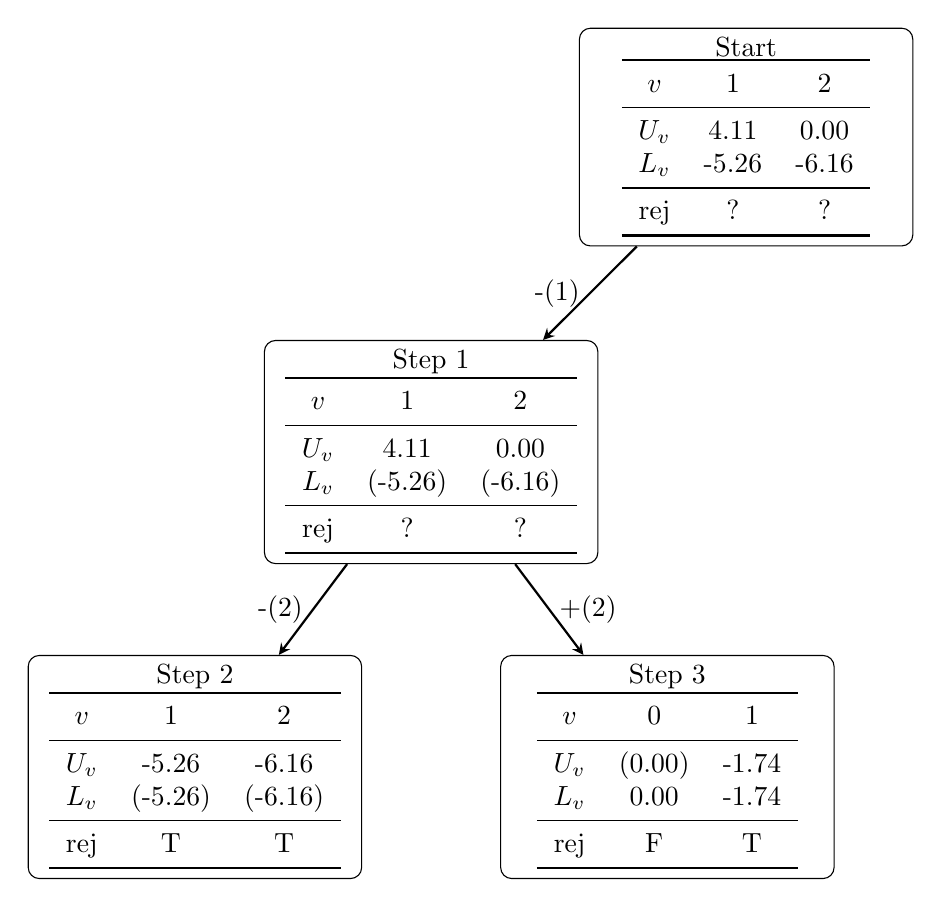
\begin{tikzpicture}[node distance = 4cm]
\node (n0) [c-rectangle2] {Start\\
\begin{tabular}{ccc}
\toprule
$v$ & 1 & 2 \\
\midrule
$U_v$ & 4.11 & 0.00\\
$L_v$ & -5.26 & -6.16\\
\midrule
rej & ? & ?\\
\bottomrule
\end{tabular}
};
\node (n1) [c-rectangle2, below of=n0, xshift=-4cm] {Step 1\\
\begin{tabular}{ccc}
\toprule
$v$ & 1 & 2 \\
\midrule
$U_v$ & 4.11 & 0.00\\
$L_v$ & (-5.26) & (-6.16)\\
\midrule
rej & ? & ?\\
\bottomrule
\end{tabular}
};
\node (n2) [c-rectangle2, below of=n1, xshift=-3cm] {Step 2\\
\begin{tabular}{ccc}
\toprule
$v$ & 1 & 2 \\
\midrule
$U_v$ & -5.26 & -6.16\\
$L_v$ & (-5.26) & (-6.16)\\
\midrule
rej & T & T\\
\bottomrule
\end{tabular}
};
\node (n3) [c-rectangle2, below of=n1, xshift=3cm] {Step 3\\
\begin{tabular}{ccc}
\toprule
$v$ & 0 & 1 \\
\midrule
$U_v$ & (0.00) & -1.74\\
$L_v$ & 0.00 & -1.74\\
\midrule
rej & F & T\\
\bottomrule
\end{tabular}
};
\draw [arrow] (n0) -- node[anchor=east] {-(1)} (n1);
\draw [arrow] (n1) -- node[anchor=east] {-(2)} (n2);
\draw [arrow] (n1) -- node[anchor=west] {+(2)} (n3);
\end{tikzpicture}
\caption{Branch and Bound procedure, carried out by removing the highest test statistic.}
\label{fig:bab}
\end{figure}





\newpage
\section{True Discovery Proportion}

Assume that $S$ is rejected by closed testing. The true discoveries can be estimated by analysing the subsets
\[\mathcal{Z}_z=\{Z\subseteq S\,:\, |Z|=s-z\}\]
for $z=0,\ldots,s$. Indeed, if all elements of $\mathcal{Z}_z$ are rejected by closed testing, then $TD \geq z+1$. The highest bound corresponds to the maximum $z$ value such that the condition is true.

$\mathcal{Z}_0=\{S\}$ has already been rejected. The supersets of $Z\in\mathcal{Z}_1$ are
\begin{itemize}
\item $S$ and its supersets (already rejected by the local tests);
\item supersets with the form $Z\cup V$, with $V\subseteq F\setminus S$.
\end{itemize}

Analogously, consider $\mathcal{Z}_z$, after rejecting all the elements of $\mathcal{Z}_0,\ldots,\mathcal{Z}_{z-1}$. In order to reject $Z\in\mathcal{Z}_z$, the only supersets that need to be studied have the form $Z\cup V$, with $V\subseteq F\setminus S$. We will define bounds $L_{z,v}$ and $U_{z,v}$ for the critical values of such sets.



\paragraph{Lower critical value.}  Let $\mathbf{l}_{0,v}=\mathbf{l}_v$ as defined in section 2. Let $(x_1,\ldots,x_s)$ be a permutation of the indices in $S$ such that
\[ g_{x_1}\leq g_{x_2}\leq\ldots\leq g_{x_s}.\]
For $z=1,\ldots,s$, the lower critical value is $L_{z,v}=(d_S + l_{z,v})^{(k)}$, where
\[l_{z,v}^\pi = l_{z-1,v}^\pi - d_{x_{s-z+1}}^\pi .\]
Notice that
\[d_S^\pi + l_{z,v}^\pi = \sum_{h=1}^z d_{x_h}^\pi + \sum_{h=1}^v d_{i_h}^\pi \]
is the test statistic corresponding to the set $\tilde{Z}\cup\tilde{V}=\{x_1,\ldots,x_z\}\cup\{i_1,\ldots,i_v\}$, likely to be rejected.


\paragraph{Upper critical value.} Let $\mathbf{u}_{0,v}=\mathbf{u}_v$ as defined in section 2. For each $\pi=1,\ldots,B$, let $(y_1(\pi),\ldots,y_s(\pi))$ be a permutation of the indices in $S$ such that
\[ d_{y_1(\pi)}^\pi\geq d_{y_2(\pi)}^\pi\geq\ldots d_{y_s(\pi)}^\pi .\]
Then $U_{z,v}=(d_{S} + u_{z,v})^{(k)}$ with
\[u_{z,v}^\pi = u_{z-1,v}^\pi - d_{y_{s-z+1}(\pi)}^\pi .\]
Notice that
\[d_{S}^\pi + u_{z,v}^\pi = \sum_{h=1}^z d_{y_h(\pi)}^\pi + \sum_{h=1}^v d_{j_h(\pi)}^\pi .\]

\newpage
\section{Example 2}
Considering $f=7$ predictors and $B=10$ permutations, we simulate a $B\times f$ matrix of global test statistics:

\begin{table}[h!]
\centering
\begin{tabular}{ccccccc}
\multicolumn{7}{c}{$\mathbf{G}$}\\
$(1)$ & $(2)$ & $(3)$ & $(4)$ & $(5)$ & $(6)$ & $(7)$\\
\cline{1-7}
16.68 & 11.54 & 6.12 & 0.22 & 28.42 & 9.40 & 9.36\\
0.06 & 44.17 & 0.08 & 5.33 & 0.10 & 0.56 & 1.37\\
3.07 & 12.03 & 0.83 & 6.41 & 0.69 & 0.36 & 4.33\\
30.31 & 1.81 & 8.55 & 15.99 & 1.07 & 0.26 & 1.11\\
7.45 & 28.14 & 0.48 & 0.03 & 0.22 & 1.02 & 2.87\\
0.04 & 36.87 & 0.04 & 6.13 & 1.83 & 0.02 & 2.85\\
1.82 & 1.08 & 1.52 & 4.45 & 17.68 & 1.06 & 6.00\\
26.12 & 0.27 & 0.26 & 1.06 & 1.77 & 4.07 & 0.29\\
0.37 & 2.15 & 5.83 & 3.75 & 2.71 & 4.42 & 8.47\\
0.03 & 13.97 & 8.84 & 0.66 & 1.14 & 2.41 & 24.06
\end{tabular}
\end{table}

After rejecting $S=\{5,6,7\}$ with significance level $\alpha=0.20$, we want to estimate the TDP.

We define
\begin{itemize}
\item $\mathbf{Ds}$ and $\mathbf{D}$, matrices of the centered test statistics in $S$ and $F\setminus S$, respectively;
\item $\mathbf{Rs}$ and $\mathbf{R}$, matrices obtained from $\mathbf{Ds}$ and $\mathbf{D}$ by sorting the elements within each row in decreasing order;
\item $\mathbf{Dsum}$ and $\mathbf{Rsum}$, matrices of the cumulative sums of $\mathbf{d}_S$ with $\mathbf{D}$ and $\mathbf{R}$, respectively.
\end{itemize}

Let $k=\lceil (1-\alpha) B\rceil =8$. The lower and upper critical values, $L_{z,v}$ and $U_{z,v}$, are the $k$-th ordered statistics of $\mathbf{d}_S +\mathbf{l}_{z,v}$ and $\mathbf{d}_S + \mathbf{u}_{0,v}$:
\begin{align*}
& \mathbf{d}_S +\mathbf{l}_{0,v}=\mathbf{Dsum}_{v+1} & \mathbf{d}_S + \mathbf{u}_{0,v}=\mathbf{Rsum}_{v+1} \\
& \mathbf{d}_S + \mathbf{l}_{1,v}=\mathbf{d}_S + \mathbf{l}_{0,v} - \mathbf{Ds}_{s} & \mathbf{d}_S + \mathbf{u}_{1,v}=\mathbf{d}_S + \mathbf{u}_{0,v} - \mathbf{Rs}_{s}\\
& \mathbf{d}_S + \mathbf{l}_{2,v}=\mathbf{d}_S + \mathbf{l}_{1,v} - \mathbf{Ds}_{s-1} & \mathbf{d}_S + \mathbf{u}_{2,v}=\mathbf{d}_S + \mathbf{u}_{1,v} - \mathbf{Rs}_{s-1}\\
& \ldots & \ldots
\end{align*}


\newpage

\begin{table}[h!]
\centering
%\resizebox{\textwidth}{!}{
\begin{tabular}{cccccccc}
\multicolumn{3}{c}{$\mathbf{Ds}$} & & \multicolumn{4}{c}{$\mathbf{D}$}\\
$(7)$ & $(6)$ & $(5)$ & & $(4)$ & $(3)$ & (2) & (1) \\
\cline{1-3} \cline{5-8}
0.00 & 0.00 & 0.00 &  & 0.00 & 0.00 & 0.00 & 0.00\\
-7.99 & -8.84 & -28.32 &  & 5.11 & -6.03 & 32.62 & -16.62\\
-5.02 & -9.04 & -27.72 &  & 6.18 & -5.29 & 0.48 & -13.61\\
-8.25 & -9.14 & -27.34 &  & 15.77 & 2.43 & -9.74 & 13.63\\
-6.49 & -8.38 & -28.19 &  & -0.19 & -5.63 & 16.60 & -9.23\\
-6.51 & -9.38 & -26.59 &  & 5.90 & -6.08 & 25.32 & -16.64\\
-3.36 & -8.34 & -10.74 &  & 4.23 & -4.59 & -10.46 & -14.86\\
-9.07 & -5.33 & -26.65 &  & 0.84 & -5.85 & -11.27 & 9.44\\
-0.89 & -4.98 & -25.71 &  & 3.53 & -0.28 & -9.40 & -16.31\\
14.70 & -6.99 & -27.27 &  & 0.43 & 2.72 & 2.43 & -16.65\\
\end{tabular}
%}
\end{table}


\begin{table}[h!]
\centering
%\resizebox{\textwidth}{!}{
\begin{tabular}{cccccccc}
\multicolumn{3}{c}{$\mathbf{Rs}$} & & \multicolumn{4}{c}{$\mathbf{R}$}\\
\cline{1-3} \cline{5-8}
0.00 (5) & 0.00 (6) & 0.00 (7) &  & 0.00 (1) & 0.00 (2) & 0.00 (3) & 0.00 (4)\\
-7.99 (7) & -8.84 (6) & -28.32 (5) &  & 32.62 (2) & 5.11 (4) & -6.03 (3) & -16.62 (1)\\
 -5.02 (7) & -9.04 (6) & -27.72 (5) &  & 6.18 (4) & 0.48 (2) & -5.29 (3) & -13.61 (1)\\
-8.25 (7) & -9.14 (6) & -27.34 (5) &  & 15.77 (4) & 13.63 (1) & 2.43 (3) & -9.74 (2)\\
-6.49 (7) & -8.38 (6) & -28.19 (5) &  & 16.60 (2) & -0.19 (4) & -5.63 (3) & -9.23 (1)\\
-6.51 (7) & -9.38 (6) & -26.59 (5) &  & 25.32 (2) & 5.90 (4) & -6.08 (3) & -16.64 (1)\\
-3.36 (7) & -8.34 (6) & -10.74 (5) &  & 4.23 (4) & -4.59 (3) & -10.46 (2) & -14.86 (1)\\
-5.33 (6) & -9.07 (7) & -26.65 (5) &  & 9.44 (1) & 0.84 (4) & -5.85 (3) & -11.27 (2)\\
-0.89 (7) & -4.98 (6) & -25.71 (5) &  & 3.53 (4) & -0.28 (3) & -9.40 (2) & -16.31 (1)\\
14.70 (7) & -6.99 (6) & -27.27 (5) &  & 2.72 (3) & 2.43 (2) & 0.43 (4) & -16.65 (1)\\
\end{tabular}
%}
\end{table}





\begin{table}[h!]
\centering
%\resizebox{\textwidth}{!}{
\begin{tabular}{ccccccccccc}
\multicolumn{5}{c}{$\mathbf{Dsum}$} & & \multicolumn{5}{c}{$\mathbf{Rsum}$}\\
\cline{1-5} \cline{7-11}
0.00 & 0.00 & 0.00 & 0.00 & 0.00 &  & 0.00 & 0.00 & 0.00 & 0.00 & 0.00 \\
-45.14 & -40.04 & -46.07 & -13.45 & -30.07 &  & -45.14 & -12.52 & -7.42 & -13.45 & -30.07\\
-41.79 & -35.61 & -40.89 & -40.41 & -54.02 &  & -41.79 & -35.61 & -35.12 & -40.41 & -54.02\\
-44.74 & -28.97 & -26.54 & -36.28 & -22.65 &  & -44.74 & -28.97 & -15.34 & -12.91 & -22.65\\
-43.07 & -43.26 & -48.90 & -32.30 & -41.53 &  & -43.07 & -26.47 & -26.66 & -32.30 & -41.53\\
-42.48 & -36.58 & -42.65 & -17.33 & -33.97 &  & -42.48 & -17.16 & -11.25 & -17.33 & -33.97\\
-22.43 & -18.20 & -22.80 & -33.26 & -48.12 &  & -22.43 & -18.20 & -22.80 & -33.26 & -48.12\\
-41.05 & -40.21 & -46.07 & -57.34 & -47.89 &  & -41.05 & -31.60 & -30.77 & -36.62 & -47.89\\
-31.58 & -28.05 & -28.33 & -37.73 & -54.04 &  & -31.58 & -28.05 & -28.33 & -37.73 & -54.04\\
-19.57 & -19.13 & -16.41 & -13.98 & -30.63 &  & -19.57 & -16.84 & -14.42 & -13.98 & -30.63\\
\end{tabular}
%}
\end{table}







\end{document}